\chapter{Pug.js}

Now we have understood how the project works, let's finally write some code.
Pug.js (abbreviated as Pug) files are translated into HTML files, they provide the basic structure of the web page. Now let's learn how to write our own web page using Pug.

\section*{Further Resources (Ch 5)}

I didn't have this piece of notes back when I first learned Pug. Here is \href{https://youtu.be/kt3cEjjkCZA}{the video}\footnote{Link: \url{https://youtu.be/kt3cEjjkCZA}{the video}} that I used to learn the basics. 

You could refer to the \href{https://www.w3schools.com/tags/default.asp}{w3schools documentation}\footnote{Link: \url{https://www.w3schools.com/tags/default.asp}} to learn how to use some more tags. There is no need to understand all the tags, , but I found the ones listed more useful than the rest. The common ones are either explained in detail in this piece of notes here. There are also more like, but unfortunately we don't have time to cover them here. The translation to Pug is well described in other parts of this chapter already.

\section{How to experiment on my code?}
\subsection*{Magic on the Pug.js website}

\textit{This method is useful when you would like to check what is the HTML code generated with the Pug code you supplied, but it cannot let you visualise the elements and see how they would actually look like in the browser.}
\vspace{6mm}

The \href{{https://pugjs.org/}}{Pug.js official website}\footnote{Link: \url{https://pugjs.org/}} contains a detailed documentation on how it is translated to HTML.

What's more valuable is its interactive translator, you can just type any Pug code on any page in the documentation, \href{https://pugjs.org/language/attributes.html}{like this one}\footnote{Link: \url{https://pugjs.org/language/attributes.html}}, type Pug code on the left box and it will translate to HTML code on the right.

\begin{figure}[h]
\centering
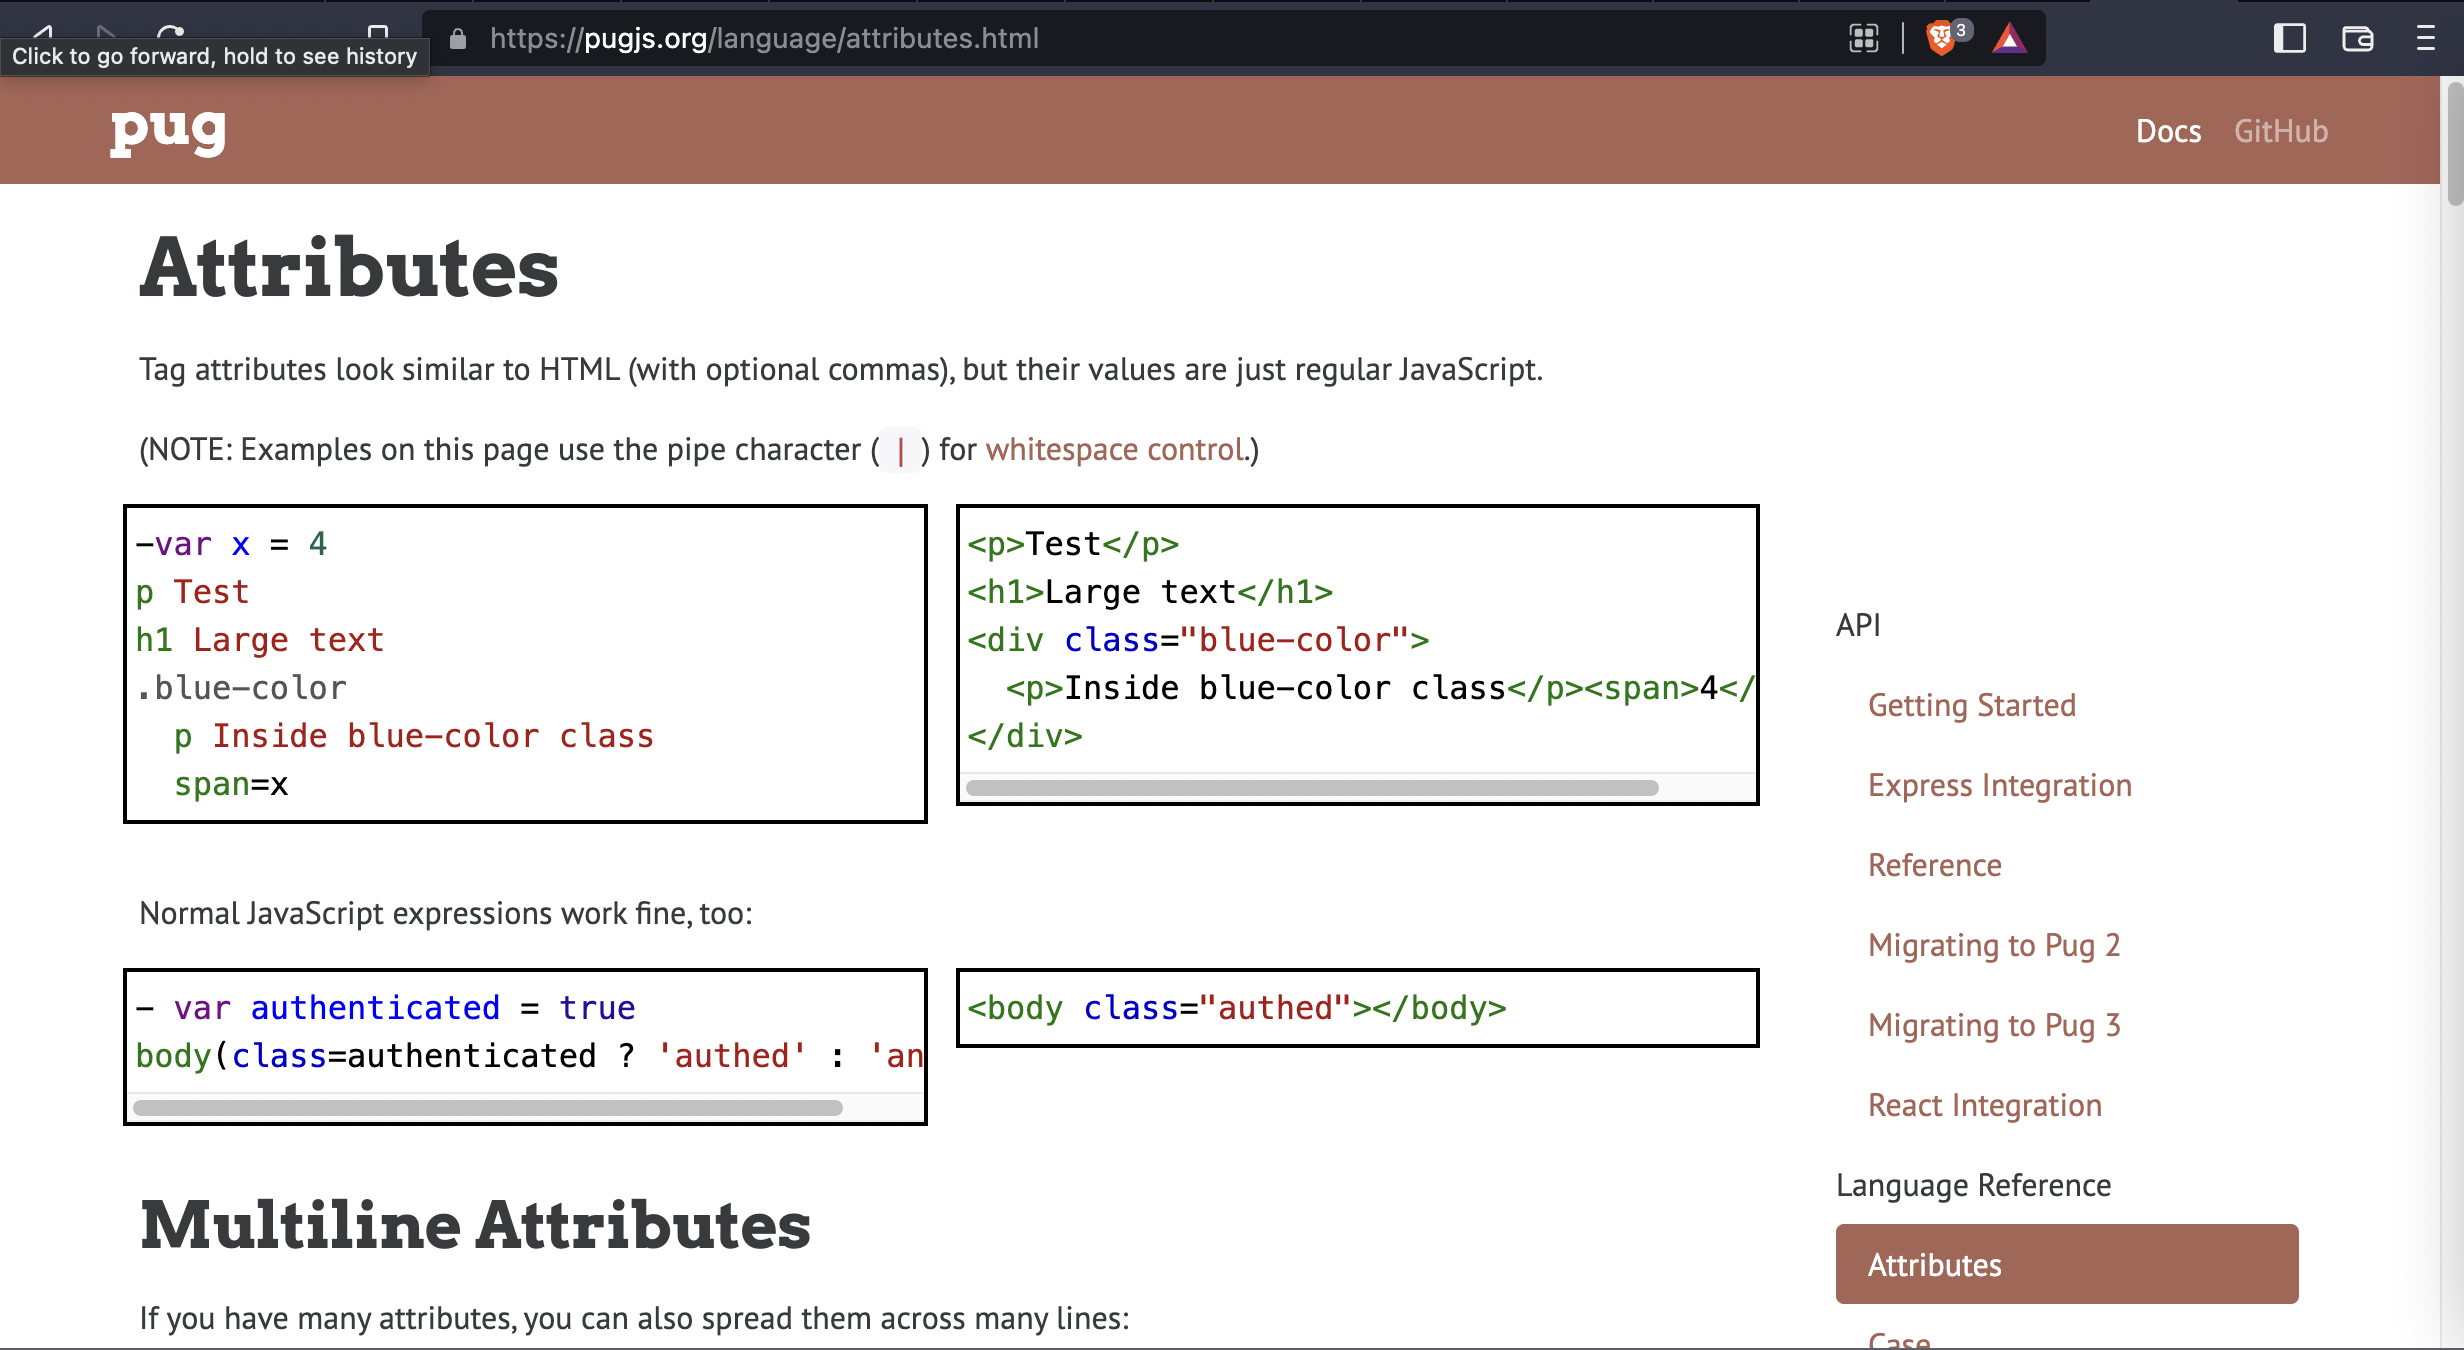
\includegraphics[width=13cm]{images/ch5-puginteractive.png}
\caption{Example usage of the interactive translator on the Pug.js official website}
\end{figure}

\subsection*{Locally on the machine}

\textit{This method is useful when you would like to visualise the elements and see how they would actually look like in the browser.}

Write the majority of your Pug code inside the \texttt{.container} class in every file under \texttt{templates/views}. 

\begin{lstlisting}[language=pug]
extends ../layouts/default

block content
	.container
		//- Your code goes here...
\end{lstlisting}

The things you write here will be translated into an HTML file matching the name of the file in the \texttt{docs} folder after you have run \texttt{npm run build}. For example, if you create a new file with the above template, called \texttt{new.pug}, then the content would appear when you open \texttt{docs/new.html} with your browser. Once again, your should NOT edit anything in the \texttt{docs} folder.

\section{General form of a Pug tag}

\begin{lstlisting}[language=pug]
a#id.class-1.class-2(href="abouts.html") Click for abouts page
\end{lstlisting}

Each line of Pug code can be divided into four sections.

\begin{enumerate}
    \item \textbf{Tag}: Specifies the type of element, can be one of the tags in the above table. The first word of the whole line would be regarded as the tag automatically by Pug.
    \item \textbf{Classes and IDs}: Give the element a reference, used in styling. We will discuss more in \cref{sec:classesids}.
    \item \textbf{Attributes}: Provides additional information for that element, in the example above, we have the \texttt{href} attribute, which tells the link to go to when we click on that element. Attributes are surrounded in parenthesis and put right after the tag, and we define them in the form of \texttt{name=value} pairs.
    \item \textbf{Plain text}: The text shown in that element. The rest of the whole line except the first word and the parenthesis following the first word.
\end{enumerate}

Classes and IDs are optional. Attributes are not needed for some of the tags. (e.g. \texttt{h1}) Plain text is not needed for some tags as well (e.g. \texttt{img}). You will see more examples along the way.

\section{Tags}

Some of you haven't coded in HTML before, so here is a quick walk-through to the basic tags, but using Pug.js syntax. Tags are like the basic building blocks of the web page, different tags corresponds to different kinds of things you can see on the web page. For example, a \texttt{p} tag denotes normal text, an \texttt{img} tag denotes an image. 
\vspace{6mm}

For those of you who have used HTML before, mind the syntactical difference, a summary of the differences will be provided in \cref{sec:pugvshtml}. 

\pagebreak

\begin{table}[H]
    \centering
    \begin{tabular}{|m{3.5em}|m{4.5em}|m{12em}|m{13em}|}
        \hline
        \textbf{Tag} & 
        Stands for &    
        Description & 
        Example in Pug
        \\ \hline \hline
        
        \texttt{p} &
        Paragraph & 
        Use this for normal text. &
        \texttt{\textbf{p} Hello world}
        \\ \hline
        
        \texttt{br} &
        Line Break & 
        Next line. e.g. to separate text into a few lines. (\cref{sec:br}) &
        \texttt{\textbf{p} this is a line \textbf{<br />} this is another line}
        \\ \hline
        
        \makecell[lb]{
            \texttt{h1}, \texttt{h2},\\ \texttt{h3}, \texttt{h4},\\ \texttt{h5}, \texttt{h6}
        } &
        \makecell[lb]{
        Header \\ 1-6 
        } & 
        Use this for titles and subheadings. \texttt{h1} is the largest, followed by \texttt{h2} and so on. &
        \makecell[lb]{
            \texttt{\textbf{h1} Header 1} \\
            \texttt{\textbf{h2} Header 2} \\
            \texttt{\textbf{h3} Header 3} \\
            ...
        }
        \\ \hline
        
        \texttt{img} &
        Image & 
        You need to specify the source \texttt{src} of the image using \textbf{attributes} (see next session). Please make sure you add your images in the \texttt{app/images} folder. (\cref{sec:img}) &
        \texttt{\textbf{img}(src="images/ bookofnumbers.jpg")}
        \\ \hline
        
        \texttt{a} &
        Anchor/ Link &
        Use this to create hyperlinks to other websites or other parts of your own website. It requires an \texttt{href} attribute indicating the destination. &
        \makecell[lb]{
            \texttt{\textbf{a}(href="abouts.html")}\\\texttt{Click for abouts page.} \\
            \texttt{\textbf{a}(href="https://www}\\\texttt{.google.com") Click}\\\texttt{for Google}
        }
        \\ \hline
        
        \makecell[lb]{
            \texttt{ul},\\\\ \texttt{ol},\\\\ \texttt{li}
        } &
        \makecell[lb]{
            unordered \\ list,\\ ordered \\ list,\\ list item
        } &
        Lists with bullet points (\texttt{ul}) or numbering (\texttt{ol}) (\cref{sec:list}) &
        \makecell[lb]{
            \texttt{\textbf{ul}} \\
            \texttt{\hspace{6mm}\textbf{li} apple} \\
            \texttt{\hspace{6mm}\textbf{li} orange} \\
            \texttt{\hspace{6mm}\textbf{li} pear} 
        }
        \\ \hline
        
        \texttt{div} &
        Division &
        It serves no purposes in adding content to the web page, but it can be used to improve organisation of your code, and it is crucial for styling. (\cref{sec:classesids}) &
        \makecell[lb]{
            \texttt{\textbf{div}} \\
            \texttt{\hspace{6mm}\textbf{h3} Numbers are} \\\texttt{\hspace{6mm}\hspace{6mm}beautiful} \\
            \texttt{\hspace{6mm}\textbf{p} - KidProf} 
        }
        \\ \hline
        
        \texttt{//-} &
        Comment &
        \tablefootnote{An alternative is \texttt{//}, using \texttt{//} means that the generated HTML file would also contain that comment, while using \texttt{//-} won't.} &
        \texttt{//- a comment} 
        \\ \hline
        
        
    \end{tabular}
\end{table}

\pagebreak

\section{Attributes}
\label{sec:img}

\textbf{Attributes} provides additional information for that element, they are surrounded in parenthesis and put right after the tag, and we define them in the form of \texttt{name=value} pairs.

Some attributes are necessary for the tags to work properly. For example, the \texttt{src} attribute that tells the \texttt{img} tag where the source of the image is. Please make sure you add your images in the \texttt{app/images} folder.
\vspace{6mm}

\begin{lstlisting}[language=pug]
img(src="images/bookofnumbers.jpg")
\end{lstlisting}

You can have more than one attributes. For example, you can specify its width and height in pixels, and also an alt text when the image cannot show properly for whatever reason.

\begin{lstlisting}[language=pug]
//- app/templates/partials/navbar.pug
img(src="images/pi-green.png" width=30 height=30 alt="pi logo")
\end{lstlisting}

However, specifying image dimensions using pixels is usually not desired because we want the image to scale based on screen width. (see \cref{sec:width}) Nonetheless, the size of the pi logo on the top left corner of the website is set using this method.
Pug uses indentation to indicate that something is in a tag

\section{How are tags put together in Pug?}

We use indentation to indicate how elements are nested. The indented tags will be surrounded by the outer tags when they got translated to HTML. We will look into some examples and also explain some of the tags in detail. 

\subsection*{Lists}
\label{sec:list}

We surround all contents of a list within a \texttt{ul} or a \texttt{ol} tag. We use \texttt{ul} (unordered list) when we need bullet points, while we use \texttt{ol} (ordered list) when we need numbering. Each bullet point is demoted by \texttt{li} (list element).

The "surrounding" I mentioned is achieved by indenting all \texttt{li} tags within the \texttt{ul} or \texttt{ol} tags.
\vspace{6mm}

\begin{lstlisting}[language=pug]
//- use of ul in the abouts page
h2 About our reference book:
ul
    li Book name: The Book of Numbers
    li Author: Tim Glynne-Jones
    li Publisher: Arcturus Publishing Limited
    li Project name: "Numbers are Fun!"
    li Topics chosen: 9, 11, 30, 365.25
    
//- A random example on the use of ol
p When you got an error message you should:
ol
    li Copy the error message
    li Go to <a href="https://www.google.com"> Google</a>
    //- The syntax used for the a tag will be discussed in the br tag section.
    li Paste and search for the error message
    li Click on the first stack overflow result
    li Copy and paste the solution
\end{lstlisting}

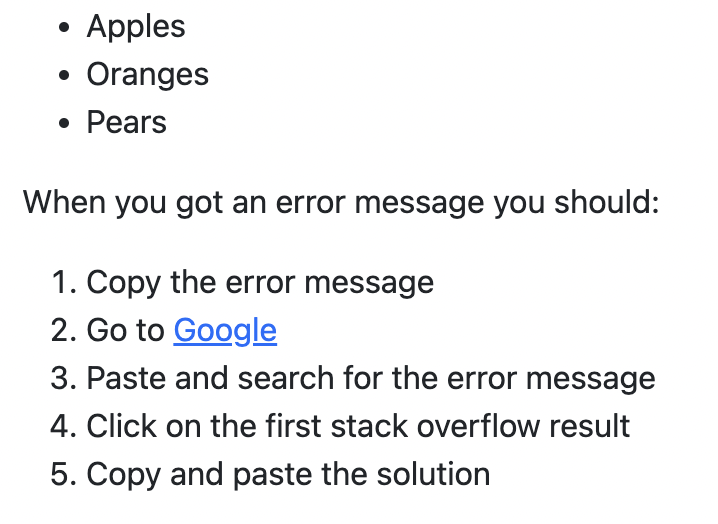
\includegraphics[width=10cm]{images/ch5-ulol.png}

\subsection*{Changing the default behaviour}

Remember that the first word in each line would be regarded as a tag. But you sometimes don't want that. 
\vspace{6mm}

For example, you might want to split the text of a \texttt{p} tag into multiple lines when the text is too long. You can actually put a \texttt{.} after the tag, and it now regards what indented within the tag as text.

\begin{lstlisting}[language=pug]
p.
	Hello, I am KidProf.
	I am a university student studying Computer Science.
	I like coding.
\end{lstlisting}


\includegraphics[width=15cm]{images/ch5-textinaline.png}

\subsection*{\texttt{br} - using normal HTML syntax in Pug}
\label{sec:br}

But when you look at the output, they are all on the same line. This is because the line breaks you made in the code is independent of the line breaks shown on the web page, \textbf{you need to explicitly use \texttt{br} tags for line breaks}. Because we are inside the \texttt{p} tag, Pug regards everything inside as text but not tags, but we can still use conventional HTML syntax to get around it.

\begin{lstlisting}[language=pug]
p.
	Hello, I am KidProf. <br />
	I am a university student studying <br />Computer Science.<br />
	I like coding.
\end{lstlisting}


\includegraphics[width=15cm]{images/ch5-textmultiplelines.png}

Alternatively, if you do not like that normal HTML code in your Pug code, you could do this instead and lead to the same result. But this is a lot of effort and affects code readability.

\begin{lstlisting}[language=pug]
p
	| Hello, I am KidProf.
	br
	| I am a university student studying
	br
	| Computer Science.
	br
	| I like coding.
\end{lstlisting}

The removal of the \texttt{.} after \texttt{p} indicates that what indented within are tags instead of plain text, so the \texttt{br} tags are registered. To indicate that the rest are plain text, the \texttt{|} character is used.

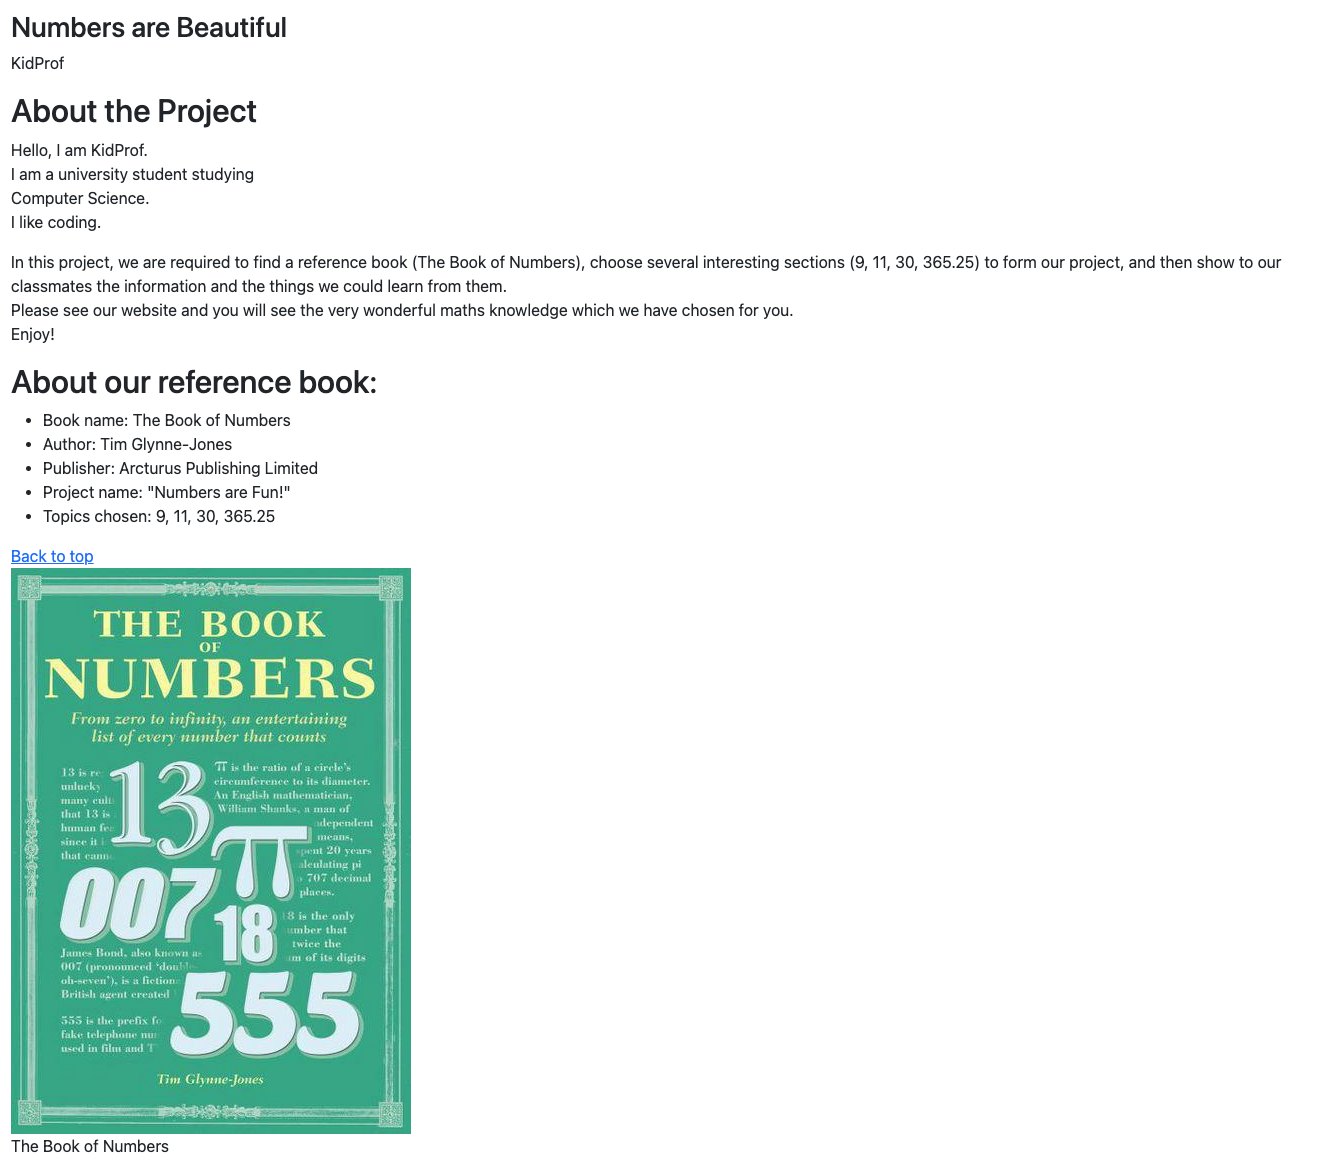
\includegraphics[width=15cm]{images/ch5-finalproduct.png}

\section{Classes and IDs}
\label{sec:classesids}

We need the notion of classes and IDs to do styling in the \hyperref[sec:ch6]{next chapter}, so that we can reference elements that we would like to style from the styling files.

We use \texttt{\#} followed by text to indicate an ID, and we use \texttt{.} followed by text to indicate a class. ID and class names must not contain spaces, it is a convention to either use camelCase or hyphens in place of spaces.
\vspace{6mm}

\begin{lstlisting}[language=pug]
//- templates/views/abouts.pug
div#quote
    h3 Numbers are Beautiful
    p KidProf
div#project-intro
    h2 About the Project
    p.
	    Hello, I am KidProf. <br />
	    I am a university student studying <br />Computer Science.<br />
	    I like coding.
    p.
        In this project, we are required to find a reference book (The Book of Numbers), choose several interesting sections (9, 11, 30, 365.25) to form our project, and then show to our classmates the information and the things we could learn from them. <br />
        Please see our website and you will see the very wonderful maths knowledge which we have chosen for you. <br />
        Enjoy!
h2 About our reference book:
div
    ul
        li.large-text Book name: The Book of Numbers
        li Author: Tim Glynne-Jones
        li Publisher: Arcturus Publishing Limited
        li.large-text Project name: "Numbers are Fun!"
        li.large-text.blue-text Topics chosen: 9, 11, 30, 365.25
    a(href="#self-intro") Back to top
div
    img#bookofnumbers(src="images/bookofnumbers.jpg")
    p.blue-text The Book of Numbers
\end{lstlisting}

In the code above we have defined a few IDs, including \texttt{\#quote} and \texttt{\#project-intro}; and also a few classes, including \texttt{.blue-text} and \texttt{.large-text}. 
\vspace{6mm}

\textbf{IDs must be unique within a page, while there can be multiple elements with the same class name in the same page.} An element can have more than one class.
\vspace{6mm}

To demonstrate one of the uses of IDs, I have included a link at the bottom of the example code. When you click on it, it brings you to the start of the page (if you zoom in large enough), to the element with ID \texttt{self-intro}. This feature does not work for classes because multiple elements can have the same class name in the same page.

The use of classes and IDs would become clearer in the \hyperref[sec:ch6]{next chapter}. We would use the classes and IDs we have defined here to reference those elements and add styles to them.\footnote{This is not the usual order of doing things. Normally, classes and IDs are added only when you want to add styles to them}

\subsection*{Classes and IDs for \texttt{div} tags}

Because \texttt{div} tags are usually associated with classes and IDs, the keyword \texttt{div} can be omitted if you have at least one class or IDs associated with it. For example, \texttt{\#quote} is equivalent to \texttt{div\#quote}.

\begin{lstlisting}[language=pug]
//- templates/views/abouts.pug
#quote
    h3 Numbers are Beautiful
    p KidProf
#project-intro
    h2 About the Project
    ...
\end{lstlisting}

\section{Summary: Pug VS HTML syntax}
\label{sec:pugvshtml}

\textit{Skip if you have not learnt HTML before, this section aims to allow HTML programmers to relate what we are learning to what they have learnt}
\vspace{6mm}

\begin{itemize}
\item Pug uses indentation to indicate that something is in a tag while HTML uses closing tags. Each line corresponds to a single tag normally. On the other hand, indentation and next lines are not important in HTML syntax.
\vspace{6mm}

\begin{lstlisting}[language=pug]
//- pug
ul
  li A
  li B
  li C
\end{lstlisting}

\begin{lstlisting}[language=html]
<!-- HTML - poorly formatted, but would still work! -->
<ul><li>A</li><li>B</li><li>C</li></ul>
\end{lstlisting}

\item All attributes should be put within parenthesis after the tag in Pug, while attributes should be put within the opening tag in HTML.
\vspace{6mm}

\begin{lstlisting}[language=pug]
//- pug
a(href="abouts.html") Click to go to the abouts page.
\end{lstlisting}

\begin{lstlisting}[language=html]
<!-- HTML -->
<a href="abouts.html">Click to go to the abouts page.</a>
\end{lstlisting}

\item Classes and IDs declarations can be simplified with Pug using the syntax shown in \cref{sec:classesids}. The \texttt{div} keyword can also be omitted when used with classes and IDs.
\vspace{6mm}

\begin{lstlisting}[language=pug]
//- pug
a#abouts-link.class1.class2(href="abouts.html") Click to go to the abouts page.
\end{lstlisting}

\begin{lstlisting}[language=html]
<!-- HTML -->
<a href="abouts.html" id="abouts-link" class="class1 class2">Click to go to the abouts page.</a>
\end{lstlisting}

\end{itemize}